% \documentclass[paper=a4, fontsize=11pt]{scrartcl} % A4 paper and 11pt font size
\documentclass[11pt, a4paper]{book}
\usepackage[T1]{fontenc} % Use 8-bit encoding that has 256 glyphs
\usepackage[utf8]{inputenc}
\usepackage{fourier} % Use the Adobe Utopia font for the document - comment this line to return to the LaTeX default
\usepackage{listings} % para insertar código con formato similar al editor
\usepackage[spanish, es-tabla]{babel} % Selecciona el español para palabras introducidas automáticamente, p.ej. "septiembre" en la fecha y especifica que se use la palabra Tabla en vez de Cuadro
\usepackage{url} % ,href} %para incluir URLs e hipervínculos dentro del texto (aunque hay que instalar href)
\usepackage{graphics,graphicx, float} %para incluir imágenes y colocarlas
\usepackage[gen]{eurosym} %para incluir el símbolo del euro
\usepackage{cite} %para incluir citas del archivo <nombre>.bib
\usepackage{enumerate}
\usepackage{hyperref}
\usepackage{graphicx}
\usepackage{tabularx}
\usepackage{booktabs}

\usepackage[table,xcdraw]{xcolor}
\hypersetup{
	colorlinks=true,	% false: boxed links; true: colored links
	linkcolor=black,	% color of internal links
	urlcolor=cyan		% color of external links
}

\renewcommand{\familydefault}{\sfdefault}
\usepackage{fancyhdr} % Custom headers and footers
\pagestyle{fancyplain} % Makes all pages in the document conform to the custom headers and footers
\fancyhead[L]{} % Empty left header
\fancyhead[C]{} % Empty center header
\fancyhead[R]{Ángel Gómez Martín} % My name
\fancyfoot[L]{} % Empty left footer
\fancyfoot[C]{} % Empty center footer
\fancyfoot[R]{\thepage} % Page numbering for right footer
%\renewcommand{\headrulewidth}{0pt} % Remove header underlines
\renewcommand{\footrulewidth}{0pt} % Remove footer underlines
\setlength{\headheight}{13.6pt} % Customize the height of the header
\setlength{\parskip}{1ex}

\usepackage{titlesec, blindtext, color}
\definecolor{gray75}{gray}{0.75}
\newcommand{\hsp}{\hspace{20pt}}
\titleformat{\chapter}[hang]{\Huge\bfseries}{\thechapter\hsp\textcolor{gray75}{|}\hsp}{0pt}{\Huge\bfseries}
\setcounter{secnumdepth}{4}
\usepackage[Lenny]{fncychap}


\begin{document}
	\begin{titlepage}
\newlength{\centeroffset}
\setlength{\centeroffset}{-0.5\oddsidemargin}
\addtolength{\centeroffset}{0.5\evensidemargin}
\thispagestyle{empty}

\noindent\hspace*{\centeroffset}\begin{minipage}{\textwidth}

\centering
\includegraphics[width=0.9\textwidth]{logos/logo_ugr.jpg}\\[1.4cm]

\textsc{ \Large TRABAJO FIN DE MÁSTER\\[0.2cm]}
\textsc{ GRADO EN INGENIERÍA INFORMÁTICA}\\[1cm]

{\Huge\bfseries Matroos \\}
\noindent\rule[-1ex]{\textwidth}{3pt}\\[3.5ex]
{\large\bfseries Creación, configuración y despliegue de bots en \textit{Discord} }
\end{minipage}

\vspace{2.5cm}
\noindent\hspace*{\centeroffset}
\begin{minipage}{\textwidth}
\centering

\textbf{Autor}\\ {Ángel Gómez Martín}\\[2.5ex]
\textbf{Director}\\ {Juan Julián Merelo Guervós}\\[2cm]
\includegraphics[width=0.3\textwidth]{logos/etsiit_logo.png}\\[0.1cm]
\textsc{Escuela Técnica Superior de Ingenierías Informática y de Telecomunicación}\\
\textsc{---}\\
Granada, 7 de Julio de 2022
\end{minipage}
\end{titlepage}

	\thispagestyle{empty}

\begin{center}
{\large\bfseries Matroos \\ Creación, configuración y despliegue de bots en \textit{Discord}. }\\
\end{center}
\begin{center}
Ángel Gómez Martín\\
\end{center}

%\vspace{0.7cm}

\vspace{0.5cm}
\noindent{\textbf{Palabras clave}: software libre, \textit{Discord}, bot
\vspace{0.7cm}

\noindent{\textbf{Resumen}\\
	

\cleardoublepage

\begin{center}
{\large\bfseries Matroos \\ Creación, configuración y despliegue de bots en \textit{Discord}. }\\
\end{center}
\begin{center}
	Ángel Gómez Martín\\
\end{center}
\vspace{0.5cm}
\noindent{\textbf{Keywords}: \textit{open source}, \textit{Discord}, bot
\vspace{0.7cm}

\noindent{\textbf{Abstract}\\


\cleardoublepage

\thispagestyle{empty}

\noindent\rule[-1ex]{\textwidth}{2pt}\\[4.5ex]

D. \textbf{Juan Julián Merelo Guervós}, Profesor del Departamento de Arquitectura y Tecnología de Computadores de la Universidad de Granada.

\vspace{0.5cm}

\textbf{Informa:}

\vspace{0.5cm}

Que el presente trabajo, titulado \textit{\textbf{Matroos}},
ha sido realizado bajo mi supervisión por \textbf{Ángel Gómez Martín}, y autorizo la defensa de dicho trabajo ante el tribunal
que corresponda.

\vspace{0.5cm}

Y para que conste, expiden y firman el presente informe en Granada a Julio de 2022.

\vspace{1cm}

\textbf{El director: }

\vspace{5cm}

\noindent Fdo: Juan Julián Merelo Guervós



\chapter*{Agradecimientos}

A mi tutor, JJ, por ofrecerme su ayuda, conocimientos y acertados comentarios para la realización de este proyecto.

A mis padres, Elia y Ángel, por ser un pilar fundamental y por empujarme a seguir aprendiendo cosas nuevas y a superarme cada día.

A mi hermana Cristina, por apoyarme y echarme una mano siempre que lo he necesitado.

Y a Paula, por aguantarme más que nadie todo este tiempo.


	\newpage
	\tableofcontents

	\newpage
	\listoffigures

	\listoftables 
	\newpage

	\chapter{Introducción}

\textit{Discord}\cite{discord} es una aplicación de mensajería de uso tanto personal como en empresas. Es semejante a otras herramientas que se usan en ámbitos similares, como \textit{Slack}\cite{slack} o \textit{TeamSpeak}\cite{teamspeak}, y ofrece distintos servicios de comunicación, como mensajería instantánea, chat de voz e integración con bots y videojuegos.

Estos últimos elementos son bastante importantes, ya que la integración con videojuegos ha hecho que \textit{Discord} gane visibilidad en los últimos años; y la integración con bots ha hecho que la herramienta sea una herramienta mucho más interactiva que las otras mencionadas. Más información en el estado del arte.

En concreto, este proyecto se centra en los bots, que podrían definirse como herramientas que, haciendo uso de diferentes permisos, ayudan a automatizar tareas dentro de un servidor de \textit{Discord}. Las funciones de éstos son prácticamente ilimitadas, aunque las más populares son moderación de usuarios y mensajes, música, envío de contenido, noticias o encuestas.

Usuarios más avanzados (como por ejemplo, un administrador de sistemas, o alguien que controla distintos equipos) que quieren hacer uso de este software y de su sistema de bots se ven obligados a crear distintos bots muy específicos y en ocasiones poco reutilizables. Si bien se podrían programar comandos más específicos en un único bot, sería una tarea tediosa la reutilización entre diferentes ámbitos.

Incidiendo en el aspecto de la creación de bots forma más técnica, se observa que actualmente hay tres maneras de usar bots en \textit{Discord}:

\begin{itemize}
	\item \textbf{Usar bots ya existentes}. El bot ya se encuentra creado, configurado y desplegado, y solo es necesario agregarlo al servidor para poder disfrutar de sus funcionalidades.
	\item \textbf{Crear un bot a alto nivel}. Este caso es similar al anterior, ya que se trata de un bot genérico, que es configurable en cierta medida para cada servidor. Esta configuración se hace a través de algún tipo de herramienta (generalmente una aplicación web) que permite configurar los comandos deseados. Por otro lado, ya que están pensados para un público general, las posibilidades de configuración son escasas. Suelen tener algunas plantillas de comandos básicos, como temporizadores o respuestas automáticas.
	\item \textbf{Crear un bot a bajo nivel}. En este caso el bot se crea haciendo uso de las diferentes \textit{API} que ofrece \textit{Discord} para ello y la personalización es máxima. En cambio, es más tedioso, y requiere conocimientos extra que algunos usuarios pueden no tener (como programación). Además hay que tener en cuenta que el bot debe ser desplegado manualmente, por lo que requiere un esfuerzo extra.
\end{itemize}

Además, en el caso de que se quisieran desplegar distintos bots al mismo tiempo y administrarlos desde un mismo entorno, no sería posible, ya que cada uno de estos es una instancia distinta.

Por tanto, se pretende desarrollar un \textit{framework} para crear bots de \textit{Discord} configurables que sean capaces de conectar con diferentes sistemas. La principal motivación a la hora de desarrollar este sistema es encontrar la manera de centralizar la creación y la administración de bots de este tipo, además de resolver los diferentes problemas planteados:

\begin{itemize}
	\item Dificultad al crear bots con funcionalidades específicas.
	\item Poca configuración en aspectos más técnicos, como administración de sistemas.
	\item Dificultad de manejar el despliegue de distintos bots al mismo tiempo.
\end{itemize}

Es por tanto, un software pensado para usuarios mas avanzados, ya que los usuarios con menor conocimiento de las tareas administrativas sólo hacen uso de estos bots una vez ya desplegados a través de los servidores de \textit{Discord}.

	\input{secciones/02_descripcion}
	\chapter{Estado del arte}

En este capítulo se hace un repaso de las distintas soluciones actuales que existen para la creación de bots de \textit{Discord} y la configuración de sus comandos.

\section{Definiciones previas}

Previa lectura de este capítulo es interesante conocer el significado de algunos conceptos que se usan.

\begin{itemize}
	\item \textbf{Comandos predefinidos}. Comandos de \textit{Discord} cuya funcionalidad está ya definida (y por tanto programada) y no puede ser modificada por un usuario.
	\item \textbf{Comandos personalizados}. Comandos predefinidos que pueden utilizarse con distintos parámetros para modificar su comportamiento.
	\item \textbf{Comandos reutilizables}. Comandos personalizados que una vez configurados pueden utilizarse en distintos bots.
	\item \textbf{Despliegue de un bot}. Todas aquellas tareas y actividades que hacen que un bot se encuentre disponible para ser usado por usuarios.
	\item \textbf{Control del despliegue}. Capacidad de controlar y monitorizar el despliegue de bots de \textit{Discord} en un sistema.
	\item \textbf{Comandos de moderación}. Comandos cuya funcionalidad se centra en la moderación de usuarios en los servidores de \textit{Discord}.
\end{itemize}

\section{Soluciones actuales}

Las soluciones actuales se podrían dividir en dos grupos, herramientas \textit{no-code} y herramientas que hacen uso de programación. En ambas la interacción con el sistema se hace a través de una aplicación web, y además suelen tener una apariencia muy similar. En las siguientes secciones se incluyen las herramientas con características más interesantes.

\subsection{Herramientas \textit{no-code}}

Estas herramientas permiten la creación de bots sin hacer uso de recursos de programación o similares. En general la mayoría de herramientas de este tipo tienen una serie de funcionalidades gratuitas, teniendo que adquirir un plan de pago mensual para obtener funcionalidades extra.

En la mayoría de casos estas plataformas cuentan con un único bot que se debe agregar al servidor de \textit{Discord} deseado. Esto implica que el uso del servicio de estos sólo permite el uso de un bot, configurado de forma individual para cada servidor. No se permite por tanto agregar varios bots (del mismo tipo) con distintas funcionalidades a un mismo servidor.

En ellas se puede observar también uno de los principales problemas mencionados en el capítulo anterior, la muy reducida personalización y reutilización de los comandos. En estos sistemas no se puede crear un comando específico con una funcionalidad concreta, sino que se basan en funcionalidades predefinidas no reutilizables.

\subsubsection{ProBot}

\href{https://probot.io/}{\textit{ProBot}} es sin duda la más interesante de las herramientas \textit{no-code} debido a que permite crear ilimitados comandos personalizados, siendo la principal desventaja que estos comandos son predefinidos, y no se puede cambiar su funcionalidad. Los comandos predefinidos se centran en moderación y mensajes automáticos, por lo que las posibilidades no son muy amplias.

A favor de esta herramienta también destaca que es sencilla de utilizar, la interfaz web intenta imitar a la de \textit{Discord} y es intuitiva. Por contra, es bastante intrusiva la modalidad \textit{premium}, ya que muchas secciones sugieren la compra de esta modalidad. Además es imposible controlar el despliegue del bot, y no es posible reutilizar comandos.

Sus características son:

\begin{table}[H]
    \centering
    \def\arraystretch{1.25}
    \begin{adjustbox}{max width=\textwidth}
    \begin{tabularx}{325px}{|l|L|}
    \hline
        \multicolumn{2}{|c|}{\textbf{\textit{ProBot}}} \\ \hline
    \hline
        \textbf{Tipo de comandos} & Predefinidos (ilimitados) \\ \hline
        \textbf{Comandos reutilizables} & No \\ \hline
        \textbf{Control del despliegue} & No \\ \hline
        \textbf{Número de bots} & 1, único \\ \hline
        \textbf{Experiencia} & Sencilla \\ \hline
        \textbf{Personalización extra} & Requiere \textit{premium} (mensualidades) \\ \hline
        \textbf{Características} & · Moderación\linebreak · Estadísticas\linebreak · Mensajes automáticos\linebreak · Música \\ \hline
        \textbf{Logs} & No \\ \hline
        \textbf{Premium} & \$60 al año \\ \hline
    \end{tabularx}
    \end{adjustbox}
    \caption{Características de \textit{ProBot}.}
\end{table}

\begin{figure}[H]
	\centering
	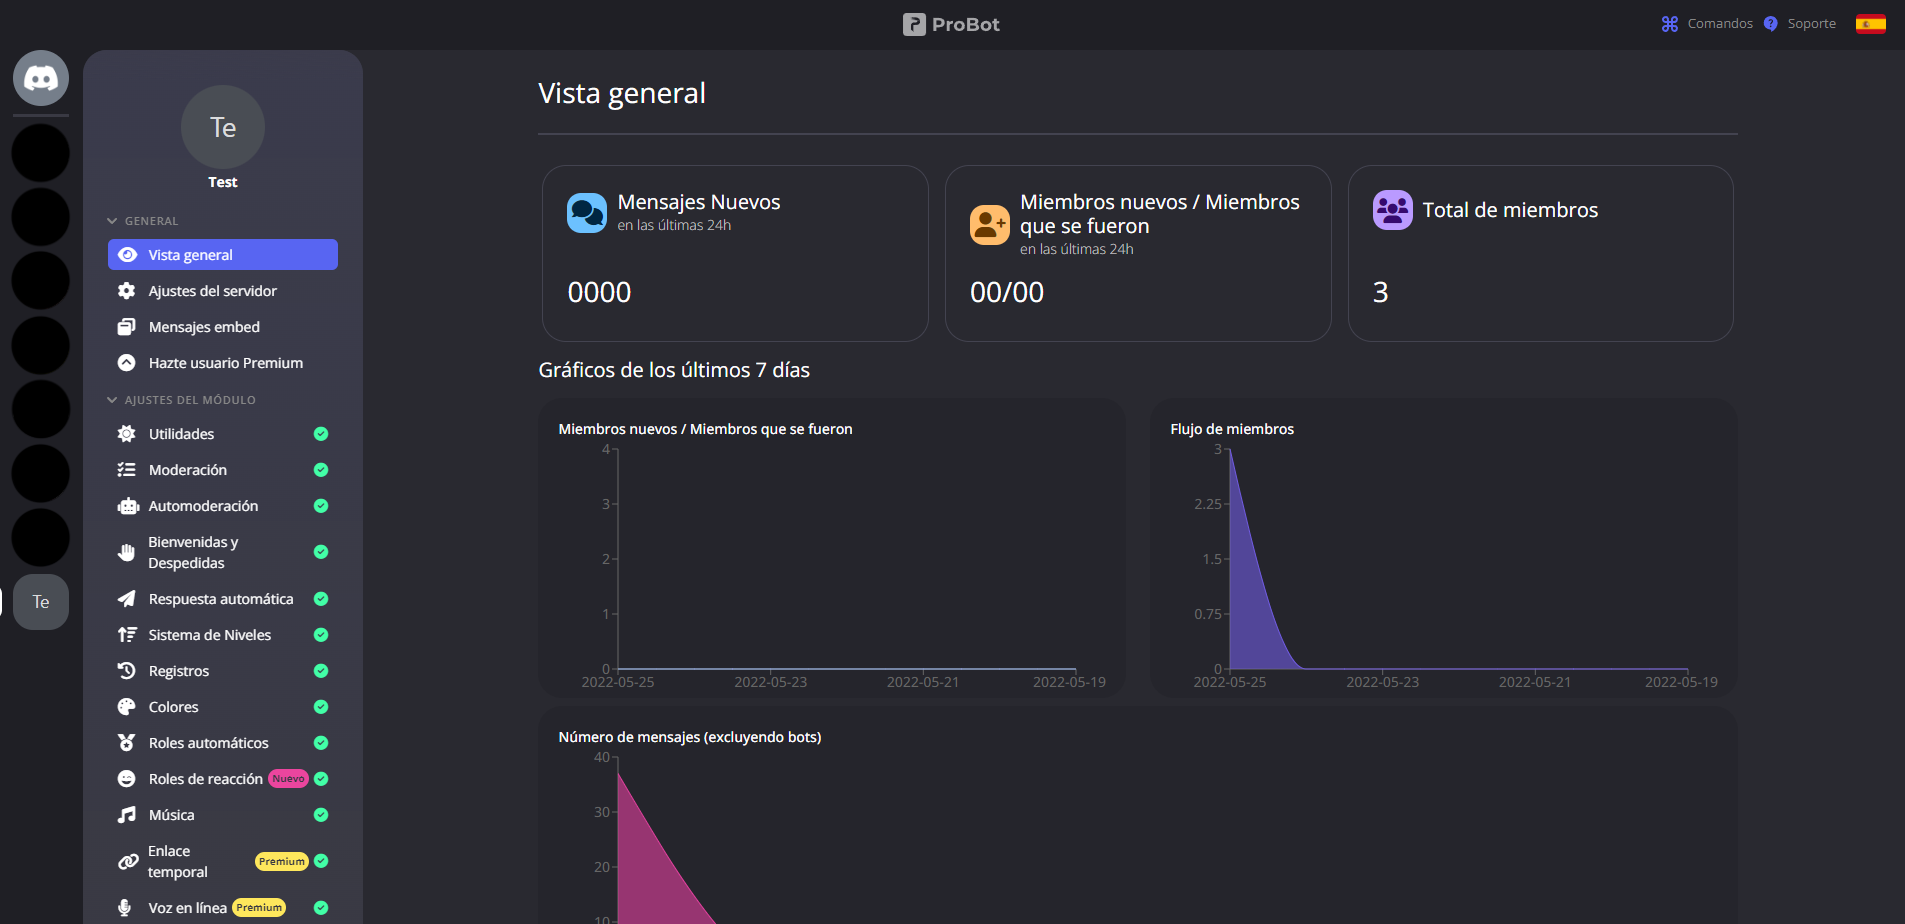
\includegraphics[width=1\textwidth]{img/probot.png}
	\caption{Interfaz web de \textit{ProBot}.}
\end{figure}

\subsubsection{Mee6}

\href{https://mee6.xyz/}{\textit{Mee6}} es otra herramienta muy similar a la anterior, siendo la principal diferencia que en este caso los comandos personalizados se limitan a 5. Por contra, tiene un mayor catálogo de funcionalidades.

De nuevo no es posible controlar el despliegue del bot, como tampoco es posible crear otro bot y agregarlo a un mismo servidor, o reutilizar comandos.

Sus características son:

\begin{table}[H]
    \centering
    \def\arraystretch{1.25}
    \begin{adjustbox}{max width=\textwidth}
    \begin{tabularx}{325px}{|l|L|}
    \hline
        \multicolumn{2}{|c|}{\textbf{\textit{Mee6}}} \\ \hline
    \hline
        \textbf{Tipo de comandos} & Predefinidos (muy limitados, 5) \\ \hline
        \textbf{Comandos reutilizables} & No \\ \hline
        \textbf{Control del despliegue} & No \\ \hline
        \textbf{Número de bots} & 1, único \\ \hline
        \textbf{Experiencia} & Sencilla \\ \hline
        \textbf{Personalización extra} & Requiere \textit{premium} (mensualidades) \\ \hline
        \textbf{Características} & · Moderación\linebreak · Estadísticas\linebreak · Mensajes automáticos\linebreak · Música\linebreak · Temporizadores\linebreak · \textit{Quiz} / \textit{Trivia} \\ \hline
        \textbf{Logs} & No \\ \hline
        \textbf{Premium} & \$50 al año / \$90 de por vida  \\ \hline
    \end{tabularx}
    \end{adjustbox}
    \caption{Características de \textit{Mee6}.}
\end{table}

\begin{figure}[H]
	\centering
	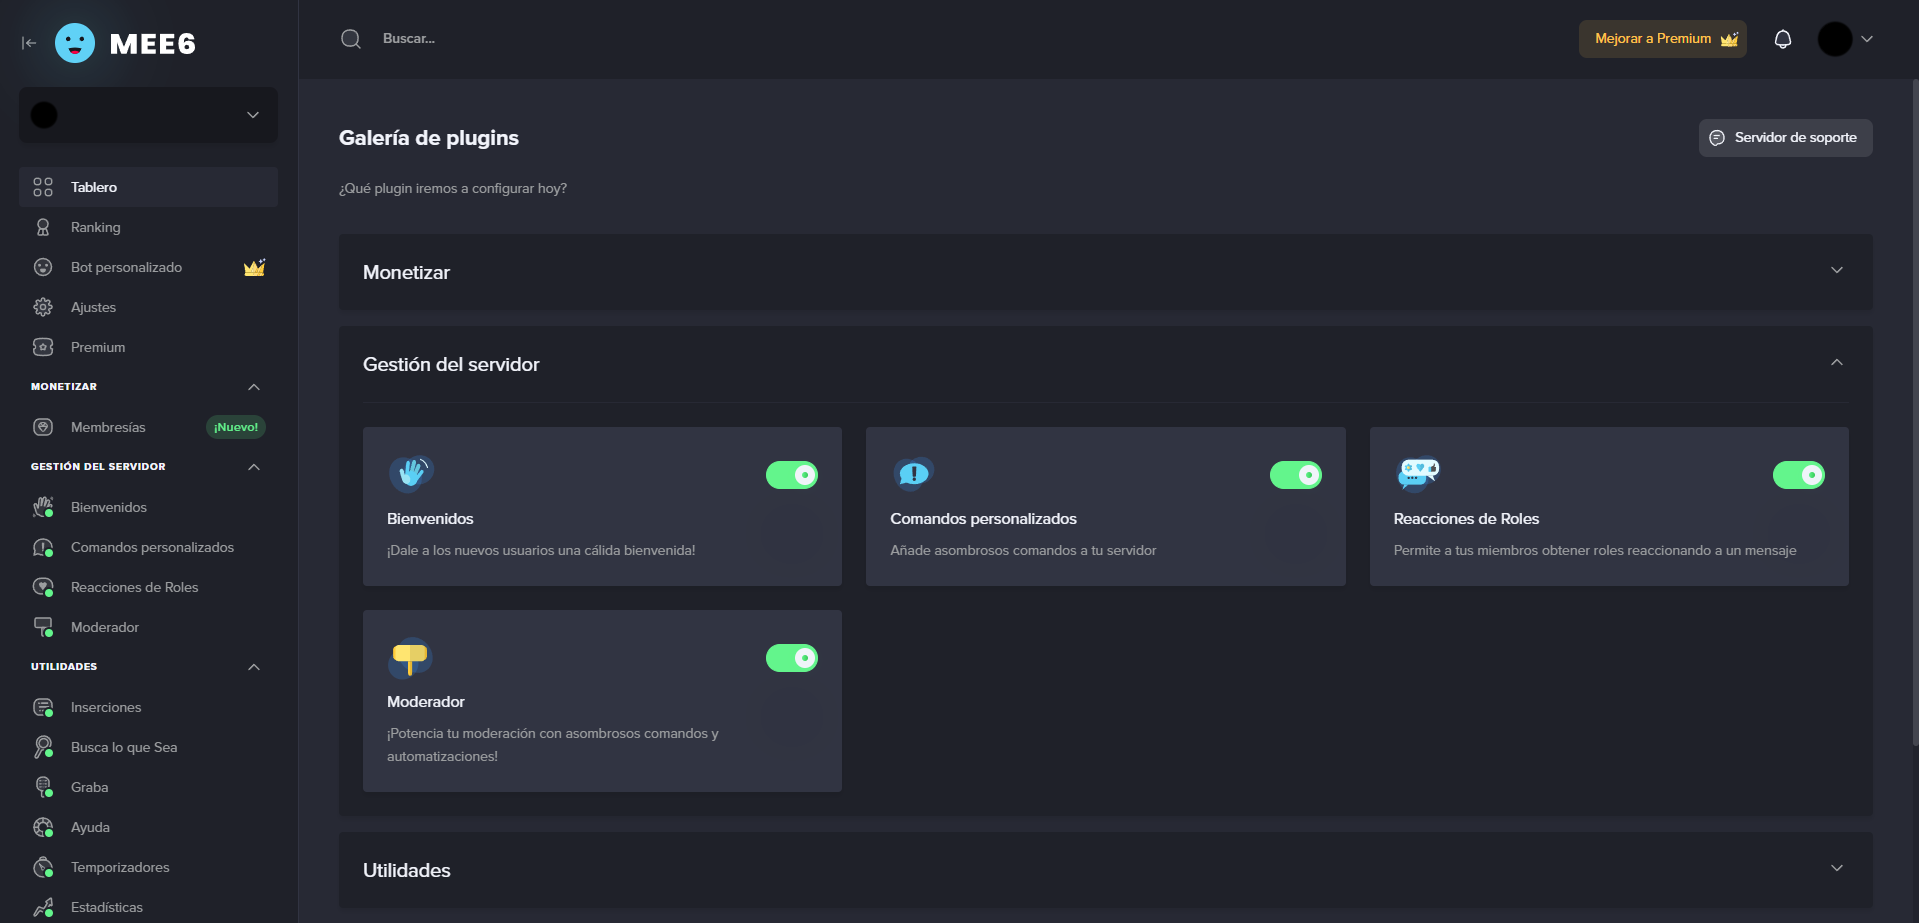
\includegraphics[width=1\textwidth]{img/mee6.png}
	\caption{Interfaz web de \textit{Mee6}.}
\end{figure}


\subsubsection{BotGhost}

\href{https://botghost.com/}{\textit{BotGhost}} es un híbrido entre \textit{ProBot} y \textit{Mee6}, ya que tiene las características comunes de ambos. La principal característica de esta herramienta es que permite crear comandos personalizados haciendo uso de una serie de módulos que se pueden interconectar para definir el ciclo de vida de un comando.

Esta característica es muy interesante, pero está muy limitada y las funcionalidades que permite realizar se resumen en envío de mensajes y tareas de moderación de usuarios muy básicas. El plan \textit{premium} sería necesario en este caso para poder sacarle partido a esta funcionalidad.

Otro aspecto interesante es que se pueden crear distintos bots, hasta 50 distintos si se opta por la opción \textit{premium}.

Sus características son:

\begin{table}[H]
    \centering
    \def\arraystretch{1.25}
    \begin{adjustbox}{max width=\textwidth}
    \begin{tabularx}{325px}{|l|L|}
    \hline
        \multicolumn{2}{|c|}{\textbf{\textit{BotGhost}}} \\ \hline
    \hline
        \textbf{Tipo de comandos} & Predefinidos (muy limitados, 5) \\ \hline
        \textbf{Comandos reutilizables} & Sí \\ \hline
        \textbf{Control del despliegue} & No (Sólo encendido y apagado) \\ \hline
        \textbf{Número de bots} & 1, único (50 con \textit{premium}) \\ \hline
        \textbf{Experiencia} & Compleja \\ \hline
        \textbf{Personalización extra} & Requiere \textit{premium} (mensualidades) \\ \hline
        \textbf{Características} & · Moderación\linebreak · Estadísticas\linebreak · Mensajes automáticos\linebreak · Temporizadores\linebreak · Integración con videojuegos\linebreak · Meteorología\linebreak · Música\linebreak · \textit{Quiz} / \textit{Trivia} \\ \hline
        \textbf{Logs} & No \\ \hline
        \textbf{Premium} & \$60 al año / \$100 de por vida \\ \hline
    \end{tabularx}
    \end{adjustbox}
    \caption{Características de \textit{BotGhost}.}
\end{table}

\begin{figure}[H]
	\centering
	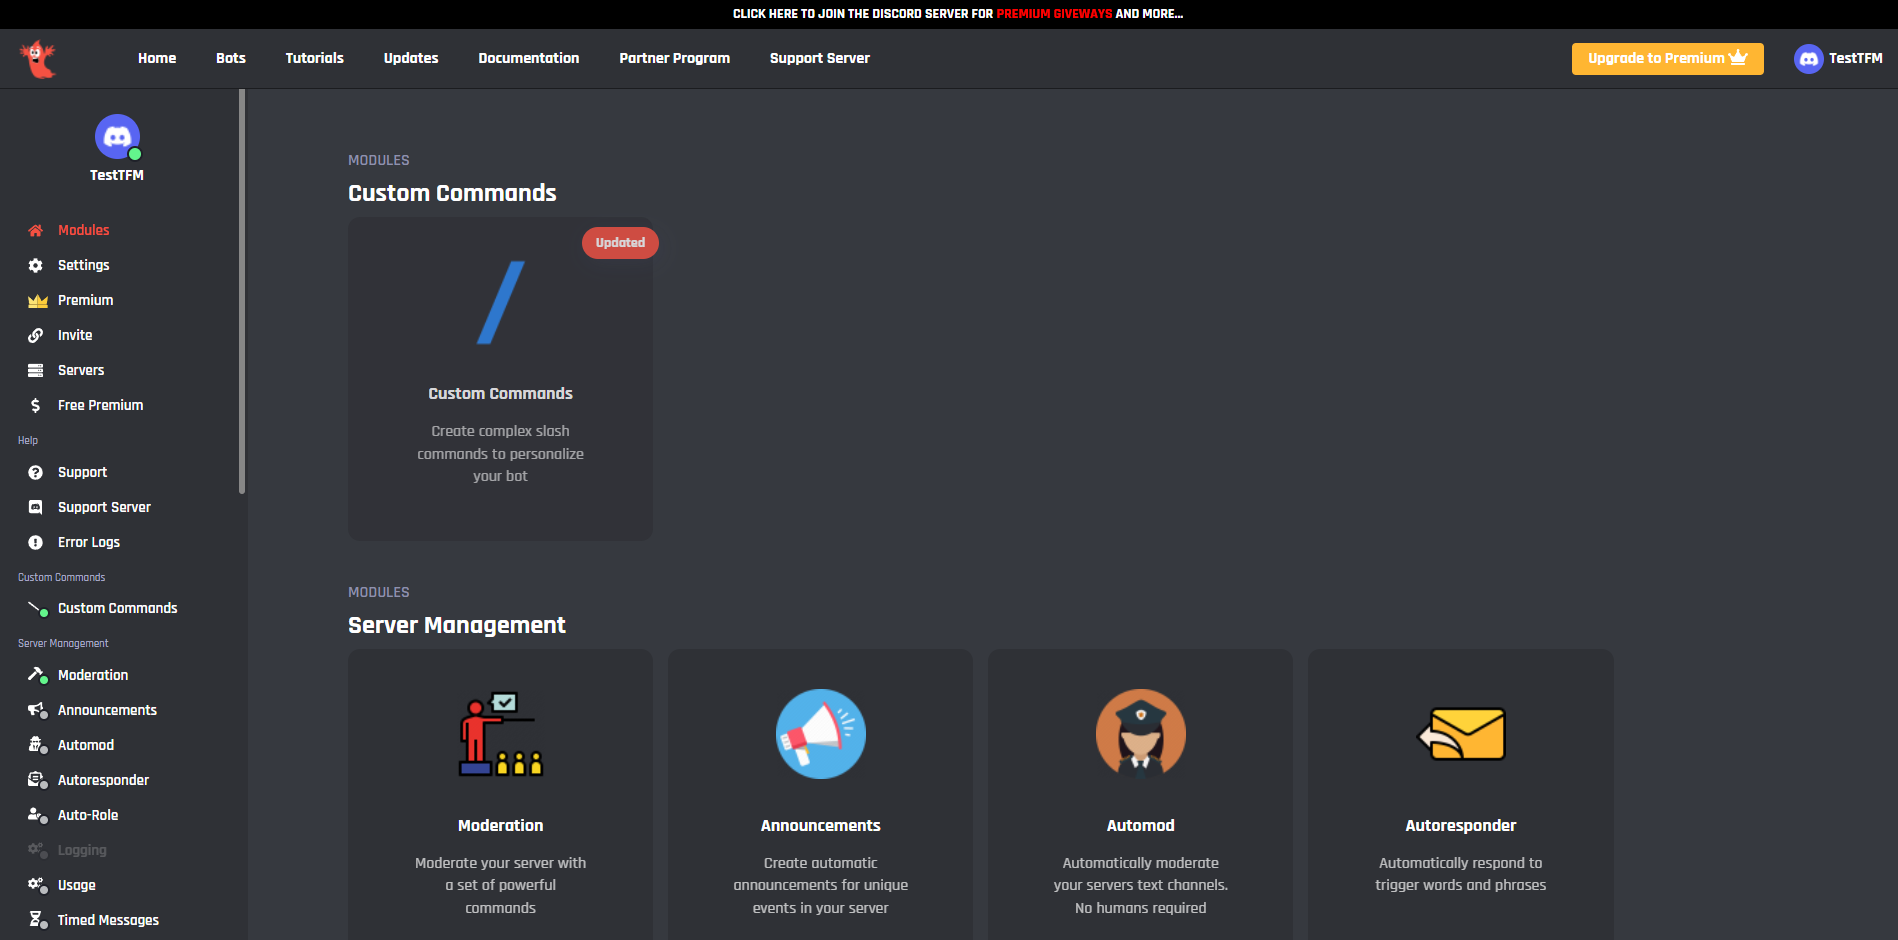
\includegraphics[width=1\textwidth]{img/botghost.png}
	\caption{Interfaz web de \textit{BotGhost}.}
\end{figure}

\subsection{Herramientas de programación}

Actualmente existen multitud de librerías para distintos lenguajes de programación que permiten interactuar con la \textit{API} de \textit{Discord} y por tanto crear un bot. Así mismo existen herramientas híbridas que permiten esta creación de una manera más sencilla.

\subsubsection{Autocode}

\href{https://autocode.com/}{Autocode} es sin duda la herramienta mas interesante que existe de esta modalidad híbrida. Realmente es una plataforma que facilita la creación y despliegue de aplicaciones y servicios web, bots, y tareas de automatización permitiendo que los usuarios escriban sólo una parte del código (\textit{JavaScript}) de estos.

De este modo el usuario sólo tiene que preocuparse por el código de la aplicación (o bot en este caso) que quiere crear, ya que del despliegue se encarga \textit{Autocode}. En su plan gratuito se pueden crear hasta 50 aplicaciones distintas, y permite la integración entre si de los distintos recursos que el usuario crea en la plataforma.

Sus características son:

\begin{table}[H]
    \centering
    \def\arraystretch{1.25}
    \begin{adjustbox}{max width=\textwidth}
    \begin{tabularx}{325px}{|l|L|}
    \hline
        \multicolumn{2}{|c|}{\textbf{\textit{Autocode}}} \\ \hline
    \hline
        \textbf{Tipo de comandos} & Predefinidos + \textit{JS} \\ \hline
        \textbf{Comandos reutilizables} & No \\ \hline
        \textbf{Control del despliegue} & Sí (limitado) \\ \hline
        \textbf{Número de bots} & 50 gratis \\ \hline
        \textbf{Experiencia} & Algo complejo \\ \hline
        \textbf{Personalización extra} & Requiere \textit{premium} (mensualidades) \\ \hline
        \textbf{Especialidad} & Despliegue general de aplicaciones \\ \hline
        \textbf{Logs} & Sí (1-30 días) \\ \hline
        \textbf{Premium} & \$180 / \$1620 al año \\ \hline
    \end{tabularx}
    \end{adjustbox}
    \caption{Resumen de soluciones actuales.}
\end{table}

\begin{figure}[H]
	\centering
	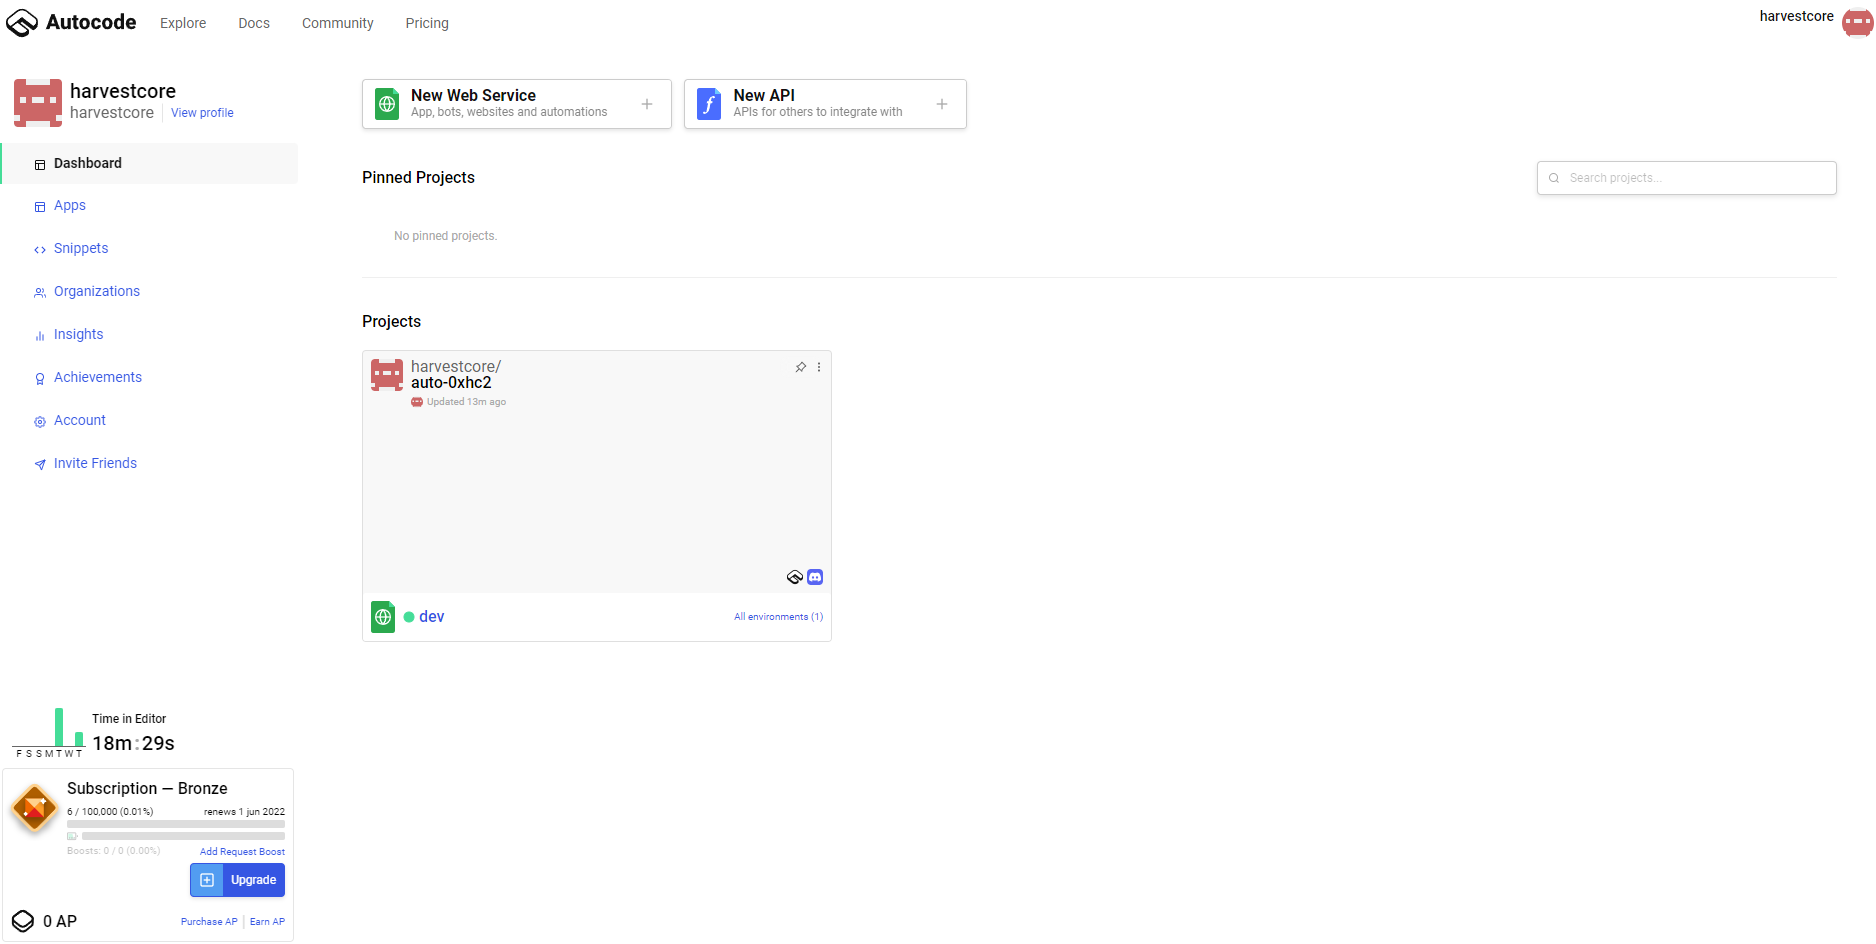
\includegraphics[width=1\textwidth]{img/autocode.png}
	\caption{Interfaz web de \textit{Autocode}.}
\end{figure}

\subsubsection{Librerías de programación}

Las librerías de programación dan libertad a la hora de crear un bot de \textit{Discord}, lo cual puede ser ideal en algunos casos. Las ventajas son obvias, ya que se puede crear cualquier tipo de comando y la reutilización es sencilla, pero en cambio, la gestión del despliegue puede ser compleja.

Por lo general todas las librerías permiten realizar casi las mismas funcionalidades, diferenciándose en aspectos como el rendimiento, la comunidad que las soporta o la facilidad de uso.

Algunos ejemplos de librerías son:

\begin{itemize}
	\item \textbf{\textit{C\#}}: \href{https://discordnet.dev/}{\textit{Discord.NET}}, \href{https://github.com/DSharpPlus/DSharpPlus}{\textit{DSharpPlus}}
	\item \textbf{\textit{Java}}: \href{https://github.com/DV8FromTheWorld/JDA}{\textit{JDA}}, \href{https://discord4j.com/}{\textit{Discord4J}}
	\item \textbf{\textit{C++}}: \href{https://dpp.dev/}{\textit{D++}}
	\item \textbf{\textit{JavaScript}}: \href{https://discord.js.org/}{\textit{discord.js}}
	\item \textbf{\textit{Golang}}: \href{https://github.com/bwmarrin/discordgo}{\textit{DiscordGo}}
	\item \textbf{\textit{Ruby}}: \href{https://github.com/shardlab/discordrb}{\textit{discordrb}}
\end{itemize}


\subsection{Comparativa de tiempos}

En esta sección se hace una comparativa del tiempo medio de desarrollo desde cero de un bot de \textit{Discord} usando las herramientas anterior mencionadas. Además se incluye tiempos de desarrollo usando tres lenguajes de programación: \textit{C\#}, \textit{JavaScript} y \textit{Python}.

Las mediciones incluyen todos los pasos necesarios para crear uno de estos bots con dos comandos personalizados. En el caso de las herramientas de programación se incluye desde la creación del proyecto hasta el despliegue (en local) de este.

Los dos comandos personalizados se han elegido al ser comunes en todas las plataformas mencionadas, además de sencillos de implementar. Son los siguientes:

\begin{itemize}
	\item Envío de un mensaje.
	\item Envío de un mensaje recurrente.
\end{itemize}

\begin{table}[H]
    \centering
    \def\arraystretch{1.25}
    \begin{adjustbox}{max width=\textwidth}
    \begin{tabularx}{200px}{|l|R|}
    \hline
        \textbf{Herramienta} & \textbf{Tiempo (en minutos)} \\ \hline
    \hline
        ProBot & 5 \\ \hline
        Mee6 & 5 \\ \hline
        BotGhost & 10 \\ \hline
    \hline
        Autocode (JS) & 45 \\ \hline
    \hline
        JS & 85 \\ \hline
        C\# & 100 \\ \hline
        Python & 80 \\ \hline
    \end{tabularx}
    \end{adjustbox}
    \caption{Comparativa de tiempos}
\end{table}

\section{Discusión}

Como se puede observar existen multitud de posibilidades a la hora de crear un bot de \textit{Discord}, y aunque cumplen lo que prometen, se centran en aspectos muy concretos dejando otros bastante desatendidos.

En las herramientas \textit{no-code} los bots se centran principalmente en tareas de moderación, envío de mensajes, estadísticas e integración con videojuegos y redes sociales. Se enfocan también en los paquetes \textit{premium}, dejando de lado detalles específicos (y que serían ideales) como:

\begin{itemize}
	\item Reutilización de comandos.
	\item No es posible crear comandos con funcionalidad específica.
	\item No se tiene control del despliegue de los bots.
	\item No se pueden crear distintos bots.
\end{itemize}

En el caso de las librerías de programación, aunque todas permiten el acceso a la \textit{API} de \textit{Discord}, cada una de ellas tiene una estructura distinta y los procedimientos para crear un bot o comandos son más o menos complejos. Si un usuario decidiese utilizarlas tendría flexibilidad completa a la hora de crear una estructura concreta, pero entonces tendría que dedicar en ese caso un tiempo necesario para diseñar algo funcional.

\textit{Autocode} es una buena alternativa a las soluciones anteriores, ya que se evita el tener que gestionar el despliegue de los bots y se eliminan algunas trabas de gestión del código, pero al igual que el uso de librerías toda la lógica recae en el usuario final. Esto puede ser útil en ciertos casos, pero no siempre.

En la comparativa de tiempos anterior se puede observar que las herramientas \textit{no-code} son las más rápidas. Esto se debe a que solo es necesario agregar el bot al servidor de \textit{Discord} deseado, y tras eso configurar de manera sencilla los comandos.

En menos de 10 minutos se puede incluir una gran cantidad de funcionalidad a un servidor de \textit{Discord} de manera gratuita, algo que puede ser muy útil para la basta mayoría de usuarios de \textit{Discord}, pero cuando se necesitan funcionalidades específicas entonces no son las ideales.

En cambio, cuando se usan herramientas que hacen uso de código, el tiempo de implementación se incrementa considerablemente. No hace justicia la comparativa, ya que en este caso se tiene que desarrollar el software por completo, por lo que es obvio que el tiempo es mayor.

En definitiva, no existe ninguna herramienta sencilla que brinde lo mejor de ambas alternativas. Por un lado se quiere facilitar la creación de bots y comandos, y el despliegue de estos. Por otro se quiere poder ampliar el repertorio de comandos disponible de manera sencilla, sin tener que desarrollar una aplicación completa para ello.

	\chapter{Planificación}

\section{Metodología de desarrollo}
\label{sec:methodology}

La metodología de desarrollo se puede definir como el proceso disciplinado que busca ser eficiente a la hora de desarrollar un software. A lo largo del tiempo han surgido numerosas metodologías que buscan mejorarse unas a otras, haciendo hincapié en elementos como coste o calidad del desarrollo. De estas, destacan los principios ágiles, los cuales se usan en multitud de entornos laborales hoy en día.

Se ha utilizado \textit{GitHub} para la gestión de un repositorio para el código, además de para utilizar las herramientas que posee que facilitan el desarrollo del software.

Tras analizar el problema se han extraído una serie de casos de uso e historias de usuario, las cuales tienen especial importancia ya que de estas dependen las características del software final. En concreto, una vez establecidas las historias de usuario han surgido una serie de tareas, las cuales se han documentado en \textit{issues} en el \href{https://github.com/harvestcore/matroos}{repositorio}.

En el caso de este proyecto el desarrollo se ha dividido en diferentes hitos, los cuales están compuestos por las anteriores tareas e historias de usuario.

El proceso a seguir para el desarrollo es sencillo. Cuando es preciso trabajar en una tarea, se crea una rama de trabajo (usualmente nombrada con el identificador de la tarea, o un texto relevante). Sobre esta rama se publican una serie de \textit{commits} que solucionan el grueso de la tarea, y posteriormente se crea un \textit{pull request} (o \textit{PR}). Esta acción permite revisar lo que se quiere unir a la rama principal de desarrollo del software, con el fin de detectar errores o iniciar discusiones si fuese necesario.

\section{Temporización}

Como se menciona en la sección de \hyperref[sec:methodology]{metodología}, el trabajo se divide en \textit{hitos} de duración variable, ya que cada uno puede requerir mayor o menor cantidad de tiempo.

En total se han creado \href{https://github.com/harvestcore/matroos/issues}{67 issues}, habiéndose completado 59 del total. El desarrollo del proyecto comenzó a finales de febrero de 2022 y ha terminado a principios de Julio de 2022.

\section{PMV y Milestones}

Un producto mínimamente viable, o \textit{PMV}, es un producto con las suficientes características capaz de atraer a los posibles clientes o usuarios tan pronto como sea posible.

Para la realización de este proyecto se ha propuesto la creación de los siguientes \textit{PMV} (o \textit{milestones}, como se llaman en \href{https://github.com/harvestcore/matroos/milestones}{GitHub}).

Los \textit{milestones} 0 a 6 son los principales del proyecto, y son los que se planea inicialmente realizar. Los \textit{milestones} 8 y 9 son adicionales, y completarían el desarrollo de todo el software incluyendo funcionalidad y características extra.

\subsection{Milestones principales}

\subsubsection{00 - Configuración del entorno, tests y CI}

Enlace en \href{https://github.com/harvestcore/matroos/milestone/3}{GitHub}.

\textbf{Versión objetivo: 0.0.1}

El \textit{PMV} incluirá:

\begin{itemize}
	\item La estructura del repositorio está definida e implementada.
	\item Los proyectos necesarios están creados y listos para continuar con el desarrollo de nuevas funcionalidades.
	\item \textit{CI} está listo para ejecutar los diferentes tests y pruebas implementadas en los distintos proyectos.
	\item La documentación hasta este punto del desarrollo está actualizada y disponible.
\end{itemize}

Decisiones técnicas y documentación adicional:

\begin{itemize}
	\item Lenguaje de programación y \textit{framework}.
	\item Integración continua.
	\item Arquitectura.
\end{itemize}

\subsubsection{01 - Modelado del dominio del problema y lógica de negocio}

Enlace en \href{https://github.com/harvestcore/matroos/milestone/12}{GitHub}.

\textbf{Versión objetivo: 0.0.2}

El \textit{PMV} incluirá:

\begin{itemize}
	\item El dominio del problema está modelado.
	\item La lógica de negocio en su forma más básica está definida.
	\item La documentación hasta este punto del desarrollo está actualizada y disponible.
\end{itemize}

Decisiones técnicas y documentación adicional:

\begin{itemize}
	\item Arquitectura.
	\item Comandos.
	\item Bots.
	\item Herramientas.
\end{itemize}

\subsubsection{02 - Gestión de comandos}

Enlace en \href{https://github.com/harvestcore/matroos/milestone/10}{GitHub}.

\textbf{Versión objetivo: 0.0.3}

Tras la finalización de este \textit{milestone}:

\begin{itemize}
	\item La estructura de los comandos está definida.
	\item El \textit{backend} cuenta con un servicio capaz de gestionar los comandos y su configuración.
	\item Los tipos de comandos básicos quedan definidos y se pueden crear nuevos comandos de estos tipos.
	\item La documentación hasta este punto del desarrollo está actualizada y disponible.
\end{itemize}

Decisiones técnicas y documentación adicional:

\begin{itemize}
	\item Arquitectura.
	\item Comandos.
\end{itemize}

\subsubsection{03 - Gestión de bots}

Enlace en \href{https://github.com/harvestcore/matroos/milestone/6}{GitHub}.

\textbf{Versión objetivo: 0.0.4}


El \textit{PMV} incluirá:

\begin{itemize}
	\item La estructura de los bots está definida.
	\item El \textit{backend} cuenta con un servicio capaz de gestionar los bots y su configuración.
	\item Es posible asociar comandos a bots.
	\item La documentación hasta este punto del desarrollo está actualizada y disponible.
\end{itemize}

Decisiones técnicas y documentación adicional:

\begin{itemize}
	\item Arquitectura.
	\item Bots.
\end{itemize}

\subsubsection{04 - Despliegue de bots en \textit{workers}}

Enlace en \href{https://github.com/harvestcore/matroos/milestone/5}{GitHub}.

\textbf{Versión objetivo: 0.0.5}


El \textit{PMV} incluirá:

\begin{itemize}
	\item Es posible desplegar (ejecutar) bots en los \textit{workers}.
	\item El \textit{backend} es capaz de comunicarse con los distintos \textit{workers}.
	\item La documentación hasta este punto del desarrollo está actualizada y disponible.
\end{itemize}

Decisiones técnicas y documentación adicional:

\begin{itemize}
	\item Lenguaje de programación y \textit{framework}.
	\item Arquitectura.
\end{itemize}

\subsubsection{05 - API REST}

Enlace en \href{https://github.com/harvestcore/matroos/milestone/7}{GitHub}.

\textbf{Versión objetivo: 0.1.0}


El \textit{PMV} incluirá:

\begin{itemize}
	\item La \textit{API Rest} está definida y los \textit{endpoints} están documentados.
	\item Es posible realizar las tareas de administración de bots y comandos haciendo uso de la API.
	\item La documentación hasta este punto del desarrollo está actualizada y disponible.
\end{itemize}

Decisiones técnicas y documentación adicional:

\begin{itemize}
	\item Lenguaje de programación y \textit{framework}.
	\item Arquitectura.
\end{itemize}

\subsubsection{06 - Despliegue en contenedores Docker}

Enlace en \href{https://github.com/harvestcore/matroos/milestone/2}{GitHub}.

\textbf{Versión objetivo: 0.2.0}


El \textit{PMV} incluirá:

\begin{itemize}
	\item El software es distribuible mediante contenedores Docker.
	\item El archivo \textit{Dockerfile} para el microservicio del \textit{backend} está disponible.
	\item El archivo \textit{Dockerfile} para el microservicio del \textit{worker} está disponible.
	\item El archivo \textit{Docker Compose} para orquestar los microservicios está disponible.
	\item La documentación hasta este punto del desarrollo está actualizada y disponible.
\end{itemize}

Decisiones técnicas y documentación adicional:

\begin{itemize}
	\item Despliegue en contenedores.
	\item Arquitectura.
\end{itemize}

\subsubsection{07 - Almacén de datos}

Enlace en \href{https://github.com/harvestcore/matroos/milestone/11}{GitHub}.

\textbf{Versión objetivo: 0.3.0}


El \textit{PMV} incluirá:

\begin{itemize}
	\item Tanto los bots como los comandos son almacenables en base de datos.
	\item La documentación hasta este punto del desarrollo está actualizada y disponible.
\end{itemize}

Decisiones técnicas y documentación adicional:

\begin{itemize}
	\item Herramientas (Base de datos).
	\item Arquitectura.
	\item Base de datos.
\end{itemize}

\subsection{Milestones adicionales}

\subsubsection{08 - Interfaz de usuario}

Enlace en \href{https://github.com/harvestcore/matroos/milestone/9}{GitHub}.

\textbf{Versión objetivo: 0.4.0}


El \textit{PMV} incluirá:

\begin{itemize}
	\item La interfaz de usuario está disponible y es capaz de realizar las tareas de creación y configuración de comandos y bots, además del despliegue de éstos en \textit{workers}.
	\item La interfaz de usuario es distribuible mediante contenedores \textit{Docker}.
	\item El archivo \textit{Dockerfile} para el microservicio está disponible.
	\item La documentación hasta este punto del desarrollo está actualizada y disponible.
\end{itemize}

Decisiones técnicas y documentación adicional:

\begin{itemize}
	\item \textit{Frontend}.
	\item Arquitectura.
\end{itemize}

	\input{secciones/05_analisis}
	\input{secciones/06_implementacion}
	\input{secciones/07_conclusiones}
	
	\newpage
	\bibliography{biblio}
	\bibliographystyle{plain}
	
\end{document}

